\fontsize{13px}{13px}\selectfont\justifying

\clearpage
\subsection{Sơ đồ hoạt động}
% https://www.uml-diagrams.org/activity-diagrams.html
\begin{figure}[h]\fontsize{13px}{13px}\selectfont
	\centering
	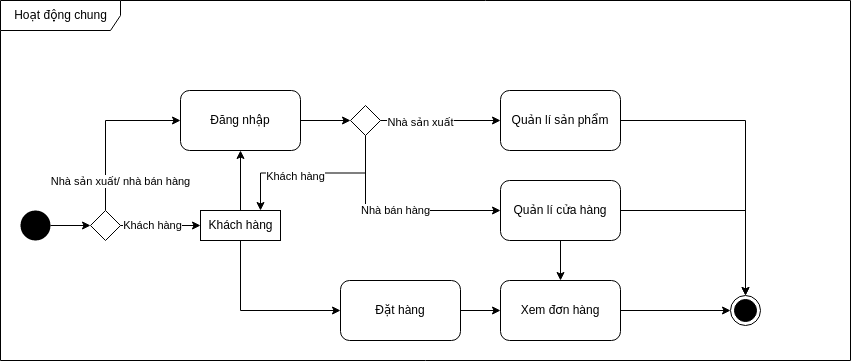
\includegraphics[width=\textwidth]{activity}
	\caption{Sơ đồ hoạt động tổng quát}
	\justifying
	Hoạt động tổng quát của hệ thống bao gồm các hành động mua hàng của khách hàng. Khách hàng mua hàng có thể đăng nhập hoặc không. Hoạt động quản lý sản phẩm, các thông tin khác của nhà sản xuất yêu cầu hoạt động đăng nhập trước đó.
\end{figure}


\begin{figure}[h!]\fontsize{13px}{13px}\selectfont
	\begin{center}	
		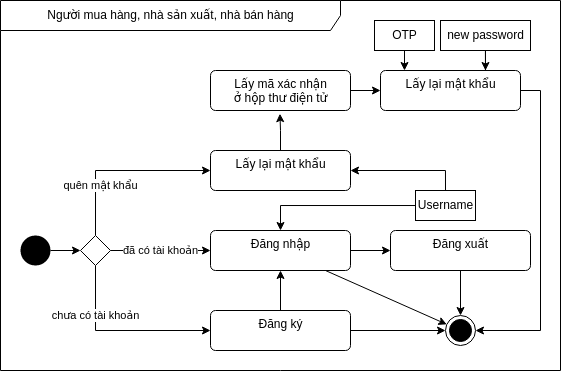
\includegraphics[width=0.8\textwidth]{activity-login}
		\caption{Sơ đồ hoạt động đăng nhập}
	\end{center}
\end{figure}


\begin{figure}[t]\fontsize{13px}{13px}\selectfont
\centering
		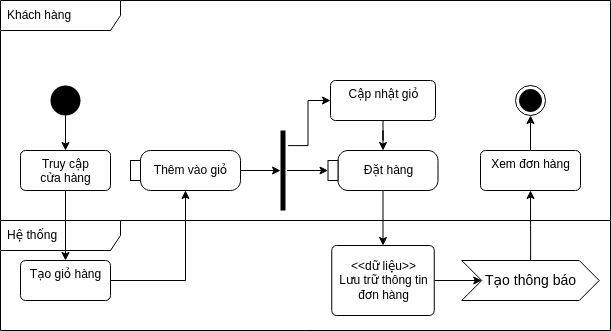
\includegraphics[width=0.7\textwidth]{activity-order}
		\caption{Sơ đồ hoạt động đặt hàng}
\justifying
Hoạt động đặt hàng được thực hiện ở phía máy khách. Khách hàng thông qua trình duyệt để thực hiện mua hàng. Hệ thống được đề cập trong sơ đồ nghĩa là phần mã javascript hoạt động dưới nền khi người dùng sử dụng trang web.
\end{figure}
\begin{figure}[btp]\fontsize{13px}{13px}\selectfont
	\begin{center}	
		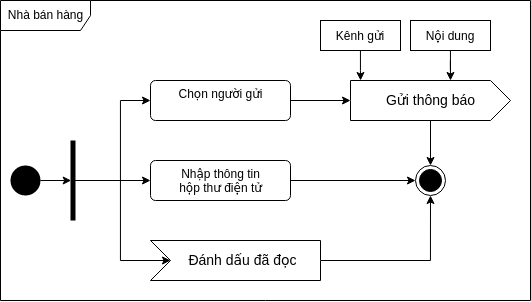
\includegraphics[width=0.7\textwidth]{activity-notification}
		\caption{Sơ đồ hoạt động thông báo}
	\end{center}
\end{figure}


\clearpage
\begin{figure}[t]\fontsize{13px}{13px}\selectfont
	\centering
		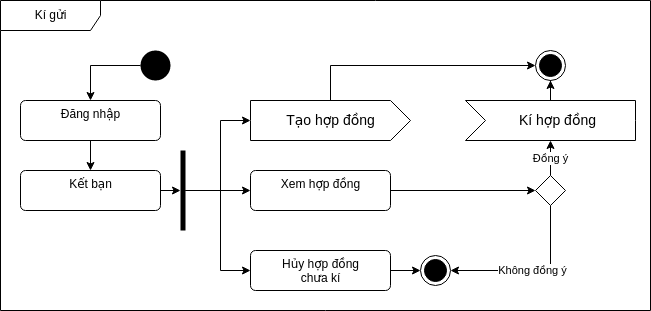
\includegraphics[width=\textwidth]{activity-contract}
		\caption{Sơ đồ hoạt động yêu cầu chia sẻ}
	\justifying
	Sơ đồ hoạt động ký hợp đồng giữa nhà bán hàng và nhà sản xuất. Sơ đồ có đề cập đến hoạt động kết bạn. Hoạt động kết bạn này sẽ được mô tả ở sơ đồ khác. Sau khi hoàn thành hoạt động lý gửi. Nhà bán hàng có thể hiển thị sản phẩm của nhà sản xuất lên trang thương mại điện tử của mình.
\end{figure}

\begin{figure}[h]\fontsize{13px}{13px}\selectfont
\centering
		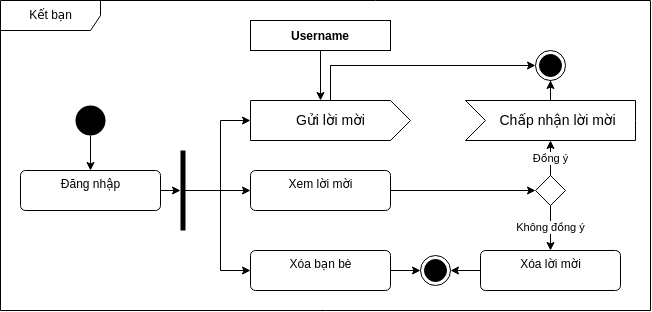
\includegraphics[width=\textwidth]{activity-relationship}
		\caption{Sơ đồ hoạt động kết bạn}
\justifying
Sau khi hoàn thành hoạt động kết bạn, nhà bán hàng có thể gửi lời mời chia sẻ sản phẩm đến các nhà sản xuất khác. Hoạt động gửi lời mời kết bạn có phân biệt người gửi và người nhận nhưng không hiển thị điều này trên giao diện.
\end{figure}
